\documentclass[12pt]{article}

\usepackage{sbc-template}

\usepackage{graphicx,url}
\usepackage{amssymb}

\usepackage[brazil]{babel}   

\usepackage[utf8]{inputenc}
     
\sloppy

\title{Sugerindo colaborações na base de doutores da Plataforma Lattes}

\author{Gabriel Dahia, Gabriel L. P. e Souza, Pedro Vidal}


\address{Departamento de Ciência da Computação -- Universidade Federal da
  (UFBA)
  \email{\{gdahia,gabriellecomt,pvidal\}@dcc.ufba.br}
}

\begin{document} 

\maketitle

% \begin{abstract}
%   This meta-paper describes the style to be used in articles and short papers
%   for SBC conferences. For papers in English, you should add just an abstract
%   while for the papers in Portuguese, we also ask for an abstract in
%   Portuguese (``resumo''). In both cases, abstracts should not have more than
%   10 lines and must be in the first page of the paper.
% \end{abstract}
     
% \begin{resumo} 
%   Este meta-artigo descreve o estilo a ser usado na confec��o de artigos e
%   resumos de artigos para publica��o nos anais das confer�ncias organizadas
%   pela SBC. � solicitada a escrita de resumo e abstract apenas para os artigos
%   escritos em portugu�s. Artigos em ingl�s dever�o apresentar apenas abstract.
%   Nos dois casos, o autor deve tomar cuidado para que o resumo (e o abstract)
%   n�o ultrapassem 10 linhas cada, sendo que ambos devem estar na primeira
%   p�gina do artigo.
% \end{resumo}


\section{Introdução}

A Plataforma Lattes, mantida pelo Conselho Nacional de Desenvolvimento Científico e Tecnológico (CNPq), corresponde a integração de bases de dados de Currículos, de Grupos de Pesquisa e de Instituições, e pauta atividades de planejamento e gestão e a formulação de políticas públicas dos órgaos governamentais brasileiros \cite{lattes-cnpq}.
Em especial, o Currículo Lattes foi criado pelo CNPq para centralizar, padronizar e disponibilizar, através da Plataforma Lattes, informações pessoais, profissionais e acadêmicas da comunidade científica brasileira \cite{sucupira}.
Essas informações são fornecidas pelos próprios autores dos currículos \cite{sucupira} e oferece grande abrangência e confiabilidade, sendo hoje adotado pela maioria das instituições de fomento, universidades e instituições de pesquisa do Brasil \cite{lattes-cnpq}.

Apesar da riqueza e potencial dessa base de dados, o CNPq impõe restrições ao acesso dessas informações, limitando o seu estudo \cite{lattes-dataset}.
Com intuito de disseminar o conteúdo da Plataforma Lattes, foi publicado o conjunto de dados \emph{LattesDoctoralDataset} \cite{lattes-dataset}.
Esta base contém dados a respeito do número e do tipo de publicações feitas, das colaborações entre pesquisadores, da atuação profissional e da formação acadêmica dos 265.187 doutores que possuem currículo publicado na plataforma, formatados em arquivos de formato \textit{comma separated values} (CSV).

O foco desse trabalho, portanto, é realizar uma análise das colaborações relatadas pelos doutores no conjunto da \emph{LattesDoctoralDataset}, com um enfoque na possibilidade de sugerir ou prever novas colaborações com base nas informações fornecidas e nas colaborações preexistentes.
Para isso, foram utilizadas técnicas de mineração de texto para pré-processamento da base e técnicas de mineração de dados para a obtenção de novas possíveis colaborações.

O restante desse relatório é dividido da seguinte forma: a seção \ref{sec:dataset} entra em mais detalhes sobre a composição do conjunto de dados utilizados, a seção \ref{sec:methods} detalha a metodologia empregada, incluindo pré-processamento, divisão da base e experimentos, a seção \ref{sec:results} apresenta os resultados e sua discussão, e a seção \ref{sec:conclusion} apresenta as conclusões do trabalho.

\section{Análise de \emph{LattesDoctoralDataset}}
\label{sec:dataset}

A base de dados \emph{LattesDoctoralDataset} contém informação relativa a 265.187 currículos, identificados unicamente por um identificador inteiro no intervalo \{1, 2 \dots 265.187\}.
Seus dados estão divididos em seis arquivos de formato CSV: \textit{Atuacao\_Profissional.csv}, contendo informações sobre a atuação profissional de cada doutor, como instituição atual, área de atuação e titulação máxima, \textit{Colaboracoes.csv}, contendo as colaborações relatadas entre doutores, \textit{Formacao\_Academica.csv}, contendo informações dos doutores a partir da graduação até o pós-doutorado, \textit{Producao\_Cientifica.csv}, com dados sobre a produção científica de diversos tipos relatada por cada doutor, \textit{Proficiencia.csv}, descrevendo o nível de domínio em outras línguas dos doutores,  e \textit{Orientacoes.csv}, contendo dados sobre as orientações realizadas ou andamento.
Para mais detalhes sobre a organização da base, sua coleta e conteúdo, o leitor interessado é referenciado ao artigo original de sua publicação \cite{lattes-dataset}.

Como o interesse desse trabalho está nas colaborações relatadas entre os doutores, a análise do conjunto de dados será mais aprofundada nesse quesito.
As colaborações são dadas através de um grafo simples, não direcionado - ao qual chamamos \textit{Grafo de Colaborações} - no qual os currículos são vértices e existe uma aresta de peso $w$ entre dois vértices $u$ e $v$ se os currículos de $u$ e $v$ relatam $w$ colaborações entre si.

Uma contagem simples, considerando que existem 265.187 vértices no Grafo de Colaborações, revela que se trata de um grafo esparso: existem apenas 6.902.042 arestas, quando o total possível era de $\frac{265187 \times (265187 - 1)}{2} =$ 35.161.939.891 colaborações.
Isso significa que menos de 0,02\% das possíveis colaborações entre doutores ocorreu, fundamentando o objetivo desse trabalho de sugerir novas colaborações entre doutores.

Esses dados informam também que o número médio de colaboradores (medido como o grau médio do Grafo de Colaborações) é de aproximadamente 13 por doutor, mas que, quando consideramos os 185.451 (aproximadamente 70\% do total) doutores que relataram alguma colaboração, sobe para aproximadamente 37 por doutor.

Também foram calculados o número médio de colaborações por doutor e seu desvio padrão, 93 e 356, aproximada e respectivamente, essas mesmas quantias restritas a doutores que relataram colaborações em seus currículos, respectivamente em torno de 134 e 420, e o número médio aproximado de colaborações entre colaboradores e seu desvio padrão, 2 e 4 respectivamente.
Isso revela que, apesar de a maioria dos doutores colaborarem e terem diversos colaboradores, essas colaborações são pouco produtivas.

\begin{figure}
\centering
  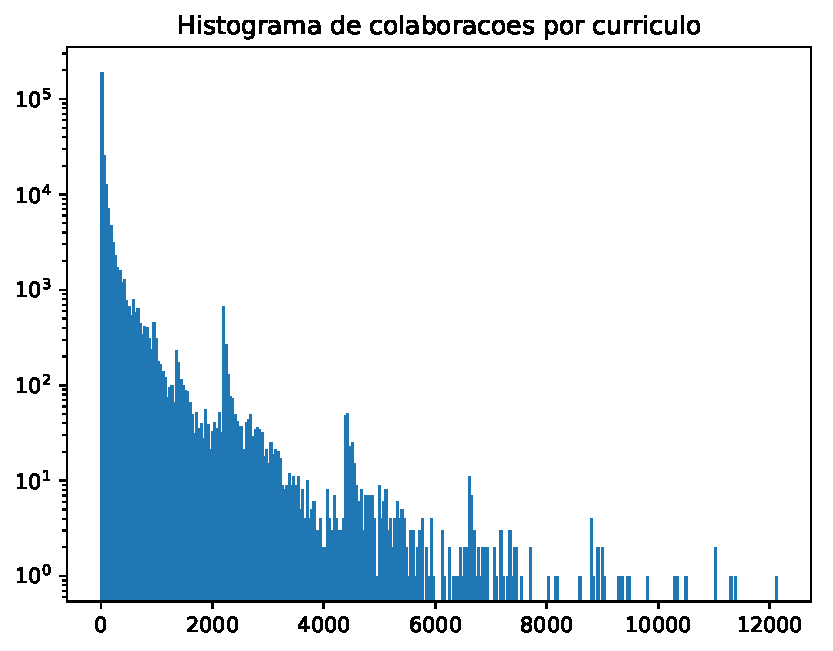
\includegraphics[width=0.45\textwidth]{graphs/degree_histogram.pdf}
  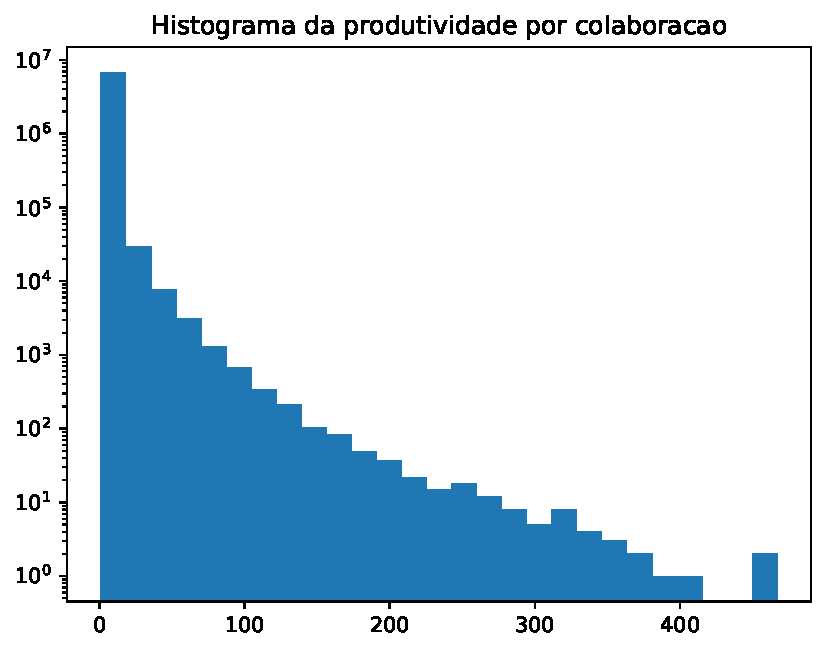
\includegraphics[width=0.45\textwidth]{graphs/weight_histogram.pdf}
  \caption{Histogramas de colaboracao por todos os currículos, à esquerda, e de produtividade por colaboração, à direita. Detalhe para o eixo vertical, em escala logaritmica.}
  \label{fig:collabs}
\end{figure}

Foram analisados também a frequência de colaboração para todos os doutores e a produtividade dessas colaborações, medida em termos de trabalhos resultantes da colaboração.
A figura \ref{fig:collabs} apresenta os histogramas resultantes dessa análise.
Desses histogramas, pode-se perceber que mesmo entre aqueles que já colaboram, prevalecem colaborações breves, com pequena produtividade, fortalecendo o argumento para a realização deste trabalho.

\section{Metodologia}
\label{sec:methods}

Para sugerir colaborações entre os doutores da base, primeiramente foi feito um pré-processamento na base de dados.
Este envolveu remover currículos com informações inconsistentes ou faltantes, agrupar as localizações e dados sobre a formação dos doutores, que são preenchidos livremente na Plataforma Lattes, utilizando técnicas de mineração de texto, e a remoção de atributos irrelevantes para a tarefa proposta.

\subsection{Pré-processamento}
\label{sec:preprocess}

O primeiro passo do pré-processamento é o descarte de currículos que não tenham colaborações relatadas ou com informações faltantes.
Nessa etapa, todo currículo com valores inválidos nos campos de atuação profissional, e, excetuando o campo ``\texttt{pos-doutorado}'', de formação acadêmica, são descartados.
Além disso, currículos que não tenham produção científica também são descartados, por entedermos que é um pré-requisito ao título de doutor a alguma produção científica.
Campos cujos significados não estão claros na formatação da base, como a seção de proficiência em línguas e os últimos campos da formação acadêmica, também foram descartados.

Os campos que podem ser especificados livremente no Currículo Lattes apresentam enorme variabilidade na maneira de especificar a mesma informação.
Por exemplo, em local de graduação, usuários podem especificar ``USP'', ``Universidade de São Paulo'' e ``Univ. de SP'' para se referir a mesma instituição.

Consideramos dois conjuntos de campos em que a variabilidade se sobressai.
O primeiro dele, a que denominou-se \texttt{lugares}, consiste de todos os campos prefixados por ``\texttt{local}'' e o campo ``\texttt{Instituicao Atual}''.
O segundo, chamado de \texttt{formacao}, contém ``\texttt{doutorado}'', ``\texttt{graduacao}'', ``\texttt{especializacao}'', ``\texttt{mestrado}'' e ``\texttt{pos-doutorado}''.

Para mitigar os efeitos da variabilidade, utilizou-se \emph{Latent Semantic Analysis} (LSA) \cite{lsa}, considerando cada entrada dos campos de ou \texttt{lugares}, ou \texttt{formacao}, a depender de qual conjunto está sendo agrupado, como um documento individual, cada valor desses campos foi transformado em um vetor no espaço $\mathbb{R}^{100}$.
Em seguida, foi aplicado o algoritmo \emph{k-Means} para classificar o conjunto de valores dos campos em 500, no caso de \texttt{formacao}, ou 3000 grupos, no caso de \texttt{lugares}.

\begin{figure}
  \centering
  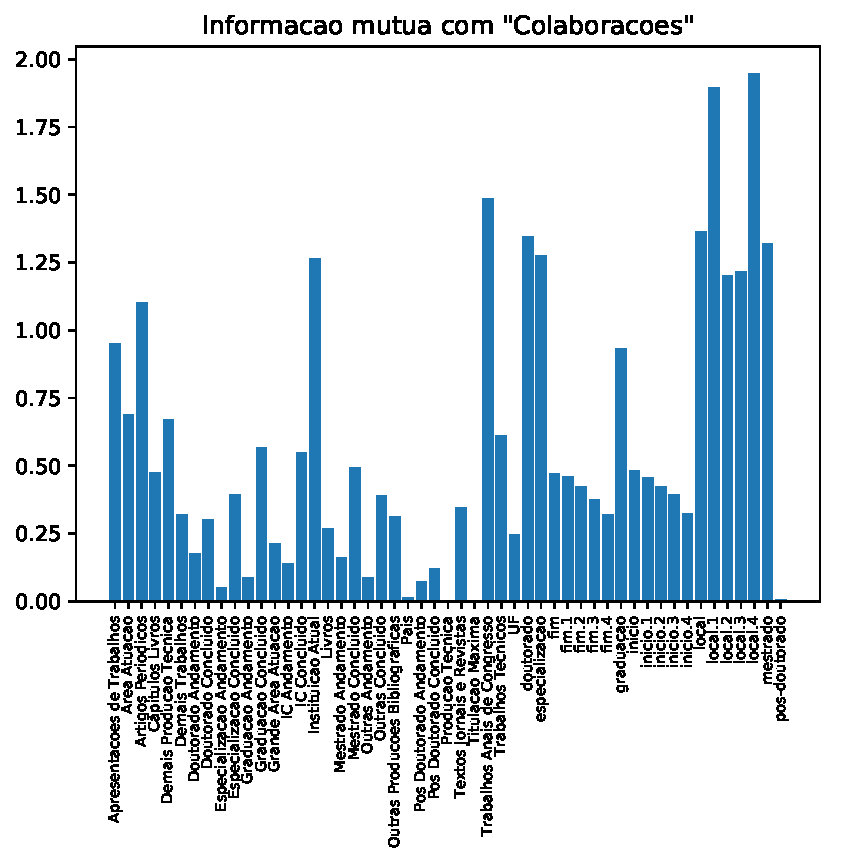
\includegraphics[width=0.7\textwidth]{graphs/mutual_information.pdf}
  \caption{Informação mútua de cada atributo com o atributo Colaborações}
  \label{fig:mutual-info}
\end{figure}

Depois de agrupados os atributos acima, calculamos a produtividade de cada doutor como a soma das produtividades de cada uma das suas colaborações e adicionamos essa informação a base como o atributo ``\texttt{Colaboracoes}''.
Utilizando esse atributo como preditor da tarefa que visa-se resolver, calculamos, entre todo outro atributo $X$ da base de dados e $Y = \texttt{Colaboracoes}$ a informação mútua $I$:

\begin{equation}
  I(X; Y) = \sum_{y \in Y} \sum_{x \in X} p(x, y) \log \left( \frac{p(x, y)}{p(x)p(y)} \right),
\end{equation}

onde $p(x, y)$ é a probabilidade conjunta de $X$ e $Y$, e $p(x)$ e $p(y)$ são, respectivamente, as probabilidades marginais de $X$ e $Y$.
Informalmente, $I(X; Y)$ mede quão independente $X$ é de $Y$ e vice-versa; isso permite quantificar dependências não-lineares entre as distribuições estudadas, diferentemente de outras métricas, como por exemplo correlação, onde apenas dependências lineares são quantificadas.

A figura \ref{fig:mutual-info} mostra a informação mútua entre os atributos e ``\texttt{Colaboracoes}'' e os outros atributos considerados.
Nessa etapa, todos os atributos $X$ tais que $I(X; Y) = 0$ foram descartados das análises subsequentes.

O resultado da etapa de pré-processamento foi uma versão da base de dados com 8.180 currículos restritos aos atributos não independentes de ``\texttt{Colaboracoes}'' e uma versão do Grafo de Colaboracões atualizada para refletir a base pré-processada, contendo 58.689 arestas.

\subsection{Modelo de mineração de dados}
\label{sec:datamine}

\section{Resultados}
\label{sec:results}

\section{Conclusão}
\label{sec:conclusion}

\bibliographystyle{sbc}
\bibliography{refs}

\end{document}
